 \chapter{Números Complexos {$\C$}}

 \vskip0.3cm
 \colorbox{azul}{
 \begin{minipage}{14.5cm}
 \begin{center}
  Definimos o conjunto dos números complexos por:
 \[\C= \{a + bi; a, b \in \R \} ,\]
 no qual temos por definição $i= \sqrt{-1}$.
 \end{center}
 \end{minipage}}
 \vskip0.3cm

 E ainda dado $z= a+bi \in \C$ chamamos o número $a$ de parte real de $z$, $Re(z)= a$ e chamamos o número $b$ de parte imaginária de $z$, $Im(z)= b$, assim se $a=0$, $z$ é um número imaginário puro, e se $b=0$ então $z$ é um número real.

 \begin{defi}
 \begin{itemize}
 \item Dois números complexos $z_1= a_1 + b_1i$ e $z_2= a_2 + b_2i$ são iguais se, e somente se, $a_1=a_2$ e $b_1= b_2$.
 \item O conjugado de um número complexo $z= a+bi$ é definido por $\overline{z}= a - bi$.
 \item Podemos representar um número complexo no plano complexo. No qual o eixo $x$ se torna o eixo real, no qual representamos a parte real do número complexo, e o eixo $y$ será o eixo imaginário, no qual representamos a parte imaginária do número complexo, assim a cada número complexo $z= a+bi$ fazemos corresponder o ponto $z= (a, b)$ do plano complexo. Por exemplo,

 \begin{figure}[H]
   \centering
   \fbox{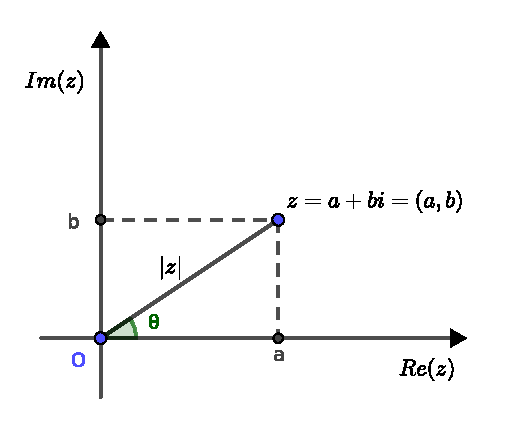
\includegraphics[width=7cm]{../../Topicos/Figuras/plano_complexo.pdf}}
   \caption{Plano complexo}
  \end{figure}

 \item O módulo ou valor absoluto de um número complexo $z= a+bi$ é definido como sendo o número real:
 \[|z|= \sqrt{a^2 + b^2},\]
 o que pode ser deduzido aplicando o teorema de pitágoras no triângulo retângulo que aparece na figura acima.
 \item No triângulo retângulo formado pelos vértices $O\hat{a}Z$, temos que:
  \begin{align*}
 & sen(\theta)= \frac{b}{|z|} & & cos(\theta)= \frac{a}{|z|} &
 \end{align*}
 No qual $\theta$ é o argumento de $z$. Note que $\theta= arctan \left( \frac{b}{a} \right)$.

 \item O número complexo tem ainda uma representação na forma polar, que é dada por:
 \[z= |z|\cdot (cos(\theta) + i sen(\theta))= |z| e^{i \theta} \]

 \end{itemize}
 \end{defi}

 Agora que temos em mãos todas as possíveis apresentações de um número complexo vamos definir as operações dentro deste conjunto.

 \textbf{Soma e subtração:} dados $z_1, z_2 \in \C$ com $z_1= a_1 + b_1i$ e $z_2= a_2 + b_2i$ temos:
 \[z_1 + z_2= (a_1 + a_2) + (b_1 + b_2)i \]
 \[z_1 - z_2= (a_1 - a_2) + (b_1 - b_2)i \]

 \textbf{Multiplicação:} dados $z_1, z_2 \in \C$ com $z_1= a_1 + b_1i$ e $z_2= a_2 + b_2i$ temos:
 \[z_1 \cdot z_2= (a_1 + b_1i) \cdot (a_2 + b_2i)= (a_1a_2 - b_1b_2) + (a_1b_2 + b_1a_2)i \]

 \textbf{Divisão:} dados $z_1, z_2 \in \C$ com $z_1= a_1 + b_1i$ e $z_2= a_2 + b_2i$ temos:
 \[z_1 \div z_2= \frac{a_1 + b_1i}{a_2 + b_2i}= \frac{a_1 + b_1i}{a_2 + b_2i} \cdot \frac{a_2 - b_2i}{a_2 - b_2i} = \frac{(a_1a_2 + b_1b_2) + (b_1a_2 - a_1b_2)i}{a_2^2 + b_2^2} \]

 \textbf{Potência:}
 \begin{align*}
 & i^0= 1 ;& & i^1= i; & & i^2= -1; & & i^3= i \cdot i^2= i \cdot (-1)= -i; & & i^4= i^2 \cdot i^2= (-1)(-1)= 1 .&
 \end{align*}

 Fórmula de Moivre
 \begin{equation}
  z^n= |z|^n[cos(n \theta) + i sen(n \theta)]
 \end{equation}

 \newpage
